% !TEX root = ../main.tex

У цьому розділі буде наведено виведення законів розподілу, що застосовуються
в задачах математичної статистики, та їх числових характеристик.

\section{Розподіл \texorpdfstring{$\chi^2$}{x2} (Пірсона)}
\noindent\textbf{Означення:}
    нехай $\xi_k \sim \mathrm{N}(a_k, \sigma_k)$, $k= 1,..., n$ --- незалежні у сукупності.
    Тоді $\xi = \sum\limits_{k=1}^n \left( \frac{\xi_k - a_k}{\sigma_k}\right)^2$ має
    розподіл \emph{$\chi^2$ (хі-квадрат, Пірсона) з $n$ ступенями вільності}.

    \noindent$\mathring{\xi}_{k} = \frac{\xi_k - a_k}{\sigma_k} \sim \mathrm{N}(0, 1)$, тому можна ще записати
    $\xi = \sum\limits_{k=1}^n (\mathring{\xi}_{k})^2$.

\noindent\textbf{Коротке позначення:} $\xi \sim \chi_n^2$, $n\in\mathbb{N}$ --- кількість ступенів вільності.

\noindent\textbf{Щільність розподілу:}
відомо, що якщо $\eta \sim \mathrm{N}(0, 1)$, то $\eta^2 \sim \Gamma\left(\frac{1}{2}, \frac{1}{2}\right)$.
Гамма-розподіл стійкий при $\beta_1 = \beta_2 = ... = \beta_n$, $\mathring{\xi}_{k}$ незалежні у сукупності,
тому $\xi = \sum\limits_{k=1}^n (\mathring{\xi}_{k})^2 \sim \Gamma\left(\frac{n}{2}, \frac{1}{2}\right) = \chi_n^2$.
\begin{equation*}
    f_{\chi_n^2}(x) = \begin{cases}
        \frac{1}{2^{\frac{n}{2}} \Gamma\left(\frac{n}{2}\right)} x^{\frac{n}{2}-1} e^{-\frac{x}{2}}, & x \geq 0 \\
        0, & x < 0
    \end{cases}
\end{equation*}

\noindent \textbf{Крива розподілу:} графіки для різних значень $n$.

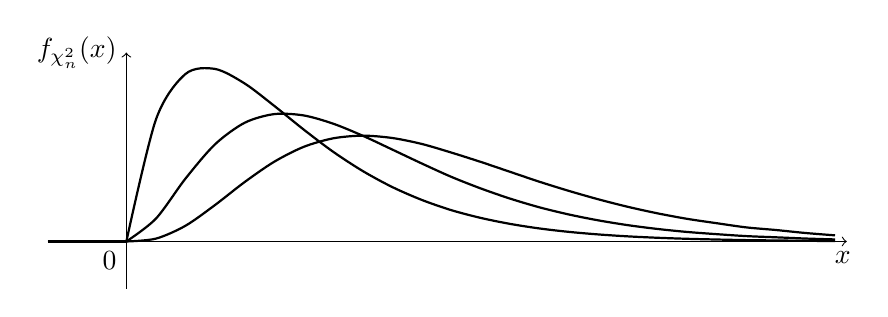
\begin{tikzpicture}[yscale = 12, xscale = 0.5, baseline={(current bounding box.center)}]
    \pgfmathsetmacro{\a}{2};
    \pgfmathsetmacro{\b}{0.5};
    \pgfmathsetmacro{\c}{3};
    \pgfmathsetmacro{\d}{4};

    \draw [->] (-2, 0) -- (18.3, 0);
    \draw [->] (0, -0.05) -- (0, 0.2);
    \draw [thick] (-2, 0) -- (0, 0);
    \draw [domain=0:18, smooth, variable = \x, thick] plot ({\x}, {\b^(\a)*\x^(\a-1)/factorial(\a-1) * e^(-\x*\b)});
    \draw [domain=0:18, smooth, variable = \x, thick] plot ({\x}, {\b^(\c)*\x^(\c-1)/factorial(\c-1) * e^(-\x*\b)});
    \draw [domain=0:18, smooth, variable = \x, thick] plot ({\x}, {\b^(\d)*\x^(\d-1)/factorial(\d-1) * e^(-\x*\b)});
    \node [below] at (18.2, 0) {$x$};
    \node [left] at (0, 0.2) {$f_{\chi_n^2}(x)$};
    \node [below left] at (0, 0) {$0$};
\end{tikzpicture}

\noindent\textbf{Числові характеристики:}
\begin{enumerate}
    \item $E\chi_n^2 = \frac{n/2}{1/2} = n$.
    \item $D\chi_n^2 = \frac{n/2}{1/4} = 2n$.
\end{enumerate}

\section{Розподіл \texorpdfstring{$\chi$}{x}}
\noindent\textbf{Означення:} нехай випадкова величина $\xi$ має розподіл $\chi_n^2$.
Тоді $\eta = \sqrt{\xi}$ має розподіл
\emph{$\chi$ (хі) з $n$ ступенями вільності}.

\noindent\textbf{Коротке позначення:} $\eta \sim \chi_n$, $n\in\mathbb{N}$ --- кількість ступенів вільності.

\noindent\textbf{Щільність розподілу:} скористаємося формулою для визначення щільності розподілу функції від
випадкової величини. $\eta = \sqrt{\xi}$, тому позначимо $\varphi(x) = \sqrt{x}$, $\varphi^{-1}(y) = y^2$,
$\left( \varphi^{-1}(y) \right)^{\prime} = 2y$.
\begin{equation*}
    f_{\chi_n}(y) = f_{\chi_n^2}\left(\varphi^{-1} (y)\right) \cdot \left|\left(\varphi^{-1} (y) \right)^{\prime}\right| =
f_{\chi_n^2}(y^2) \cdot 2y = 
\begin{cases}
    \frac{1}{2^{\frac{n}{2} - 1} \Gamma\left(\frac{n}{2}\right)} y^{n-1} e^{-\frac{y^2}{2}}, & y \geq 0 \\
    0, & y < 0
\end{cases}
\end{equation*}
\noindent\textbf{Числові характеристики:}
\begin{enumerate}
    \item $E\chi_n = \sqrt{2} \cdot \frac{\Gamma\left(\frac{n+1}{2}\right)}{\Gamma\left(\frac{n}{2}\right)}$.
    \item $D\chi_n = n - \left( E\chi_n \right)^2$.
\end{enumerate}

\begin{remark}
    Нескладно помітити, що $\chi_2$ --- це розподіл Релея.
\end{remark} 

\noindent Знайдемо ще розподіл $\zeta = \frac{\chi_n}{\sqrt{n}}$. $\varphi(y) = \frac{y}{\sqrt{n}}$,
$\varphi^{-1}(z) = z \sqrt{n}$, 
$\left( \varphi^{-1}(z) \right)^{\prime} = \sqrt{n}$.

\begin{equation*}
    f_{\frac{\chi_n}{\sqrt{n}}}(z) = f_{\chi_n}\left(\varphi^{-1} (z)\right) \cdot \left|\left(\varphi^{-1} (y) \right)^{\prime}\right| =
f_{\chi_n}(z \sqrt{n}) \cdot \sqrt{n} = 
\begin{cases}
    \frac{n^{\frac{n}{2}}}{2^{\frac{n}{2} - 1} \Gamma\left(\frac{n}{2}\right)} z^{n-1} e^{-\frac{nz^2}{2}}, & z \geq 0 \\
    0, & z < 0
\end{cases}
\end{equation*}
\begin{exercise}
    Записати числові характеристики випадкової величини, що має розподіл $\frac{\chi_n}{\sqrt{n}}$.
\end{exercise}

\section{Розподіл Стьюдента (\texorpdfstring{$t$}{t}-розподіл)}
\noindent\textbf{Означення:} якщо $\xi \sim \mathrm{N}(0, 1)$ та $\eta \sim \frac{\chi_n}{\sqrt{n}}$ незалежні,
то $\zeta = \frac{\xi}{\eta} = \frac{\xi}{\chi_n /\sqrt{n}}$ має \emph{розподіл Стьюдента з $n$ ступенями вільності}.

\noindent\textbf{Коротке позначення:} $\zeta \sim \mathrm{St}_n$, $n\in\mathbb{N}$ --- кількість ступенів вільності.

\noindent\textbf{Щільність розподілу:} скористаємося формулою для визначення щільності розподілу частки
двох незалежних НВВ.
\begin{gather*}
    f_{\mathrm{St}_n} (z) = \int\limits_0^{+\infty} x f_{\xi}(z x) f_{\frac{\chi_n}{\sqrt{n}}} (x) dx =
    \frac{1}{\sqrt{2\pi}} \cdot \frac{n^{\frac{n}{2}}}{2^{\frac{n}{2} - 1} \Gamma\left(\frac{n}{2}\right)}
    \int\limits_0^{+\infty} x e^{-\frac{z^2 x^2}{2}} x^{n-1} e^{-\frac{nx^2}{2}} dx = \\
    = \frac{n^{\frac{n}{2}}}{\sqrt{\pi} 2^{\frac{n-1}{2}} \Gamma\left(\frac{n}{2}\right)}
    \int\limits_0^{+\infty} x^n e^{-\frac{x^2}{2}(z^2+n)} dx = 
    \left[ \frac{x^2}{2} (z^2 + n) = t, x = \frac{\sqrt{2} \sqrt{t}}{\sqrt{z^2 + n}},
    dx = \frac{1}{\sqrt{2}\sqrt{z^2 + n}} \frac{dt}{\sqrt{t}}\right] = \\
    = \frac{n^{\frac{n}{2}}}{\sqrt{\pi} 2^{\frac{n-1}{2}} \Gamma\left(\frac{n}{2}\right)} \cdot
    \frac{2^{\frac{n}{2}}}{(z^2 + n)^{\frac{n}{2}}} \frac{1}{2^{\frac{1}{2}}(z^2 + n)^{\frac{n}{2}}}
    \int\limits_0^{+\infty} t^{\frac{n-1}{2}} e^{-t} dt = 
    \frac{n^{\frac{n}{2}} \Gamma\left(\frac{n+1}{2}\right)}{\sqrt{\pi} \Gamma\left(\frac{n}{2}\right)} \cdot
    \frac{1}{(z^2 + n)^{\frac{n+1}{2}}}, \; z \in \mathbb{R}
\end{gather*}
\noindent \textbf{Крива розподілу:} графіки для різних значень $n$, називаються \emph{кривими Стьюдента}.
Вони схожі на криву гауссівського розподілу, але повільніше прямують до 0 на нескінченності.

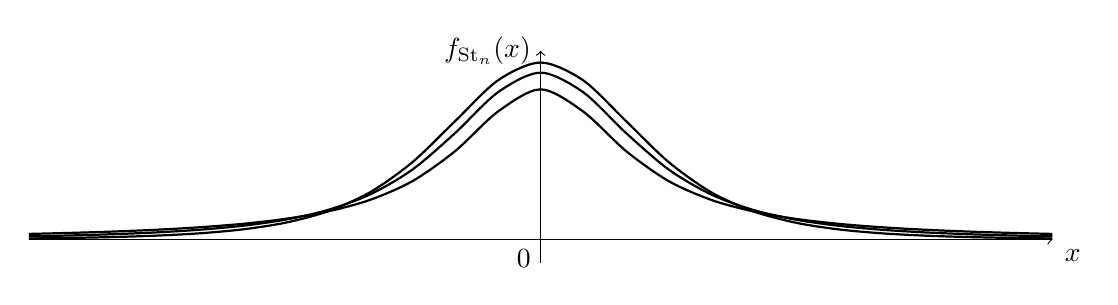
\begin{tikzpicture}[yscale = 6, xscale = 1.3, baseline={(current bounding box.center)}]
    \pgfmathsetmacro{\a}{1}; % n = 2
    \pgfmathsetmacro{\b}{12}; % n = 4
    \pgfmathsetmacro{\c}{0.318309886184}; % n = 1

    \draw [->] (-5, 0) -- (5, 0);
    \draw [->] (0, -0.05) -- (0, 0.4);
    \draw [domain=-5:5, smooth, variable = \x, thick] plot ({\x}, {\a/((2+(\x)^2)^((2+1)/2))});
    \draw [domain=-5:5, smooth, variable = \x, thick] plot ({\x}, {\b/((4+(\x)^2)^((4+1)/2))});
    \draw [domain=-5:5, smooth, variable = \x, thick] plot ({\x}, {\c/((1+(\x)^2)^((1+1)/2))});
    \node [below] at (5.2, 0) {$x$};
    \node [left] at (0, 0.4) {$f_{\mathrm{St}_n}(x)$};
    \node [below left] at (0, 0) {$0$};
\end{tikzpicture}

\noindent\textbf{Числові характеристики:}
\begin{enumerate}
    \item $E\mathrm{St}_n = 0$.
    \item $D\mathrm{St}_n = \frac{n}{n-2}$, $n>2$.
\end{enumerate}

\begin{remark}
    Нескладно помітити, що $\mathrm{St}_1$ --- це розподіл Коші.
\end{remark}

\section{Розподіл Фішера-Снедекора (\texorpdfstring{$F$}{F}-розподіл)}
\noindent\textbf{Означення:} випадкова величина $\eta = \frac{\chi_{n_1}^2/n_1}{\chi_{n_2}^2/n_2}$, чисельник
та знаменник якої незалежні, має \emph{розподіл Фішера-Снедекора з $n_1$, $n_2$ ступенями вільності}.

\noindent\textbf{Коротке позначення:} $\eta \sim \mathrm{F}(n_1, n_2)$, $n_1, n_2\in\mathbb{N}$ --- кількість ступенів вільності.

\noindent\textbf{Щільність розподілу:} скористаємося формулою для визначення щільності розподілу частки
двох незалежних НВВ. Нагадаємо, що 
$f_{\chi_n^2}(x) = \begin{cases}
    \frac{1}{2^{\frac{n}{2}} \Gamma\left(\frac{n}{2}\right)} x^{\frac{n}{2}-1} e^{-\frac{x}{2}}, & x \geq 0 \\
    0, & x < 0
\end{cases}$.

\noindentТоді $f_{\chi_n^2/n}(y) = f_{\chi_n^2}(n y) \cdot n = 
\begin{cases}
    \frac{n^{\frac{n}{2}}}{2^{\frac{n}{2}} \Gamma\left(\frac{n}{2}\right)} y^{\frac{n}{2}-1} e^{-\frac{ny}{2}}, & y \geq 0 \\
    0, & y < 0
\end{cases}$.

\begin{gather*}
    f_{\mathrm{F}(n_1, n_2)} (z) = \int\limits_0^{+\infty} x f_{\chi_{n_1}^2/n_1}(zx) f_{\chi_{n_2}^2/n_2}(x) dx = \\
    = \frac{n_1^{\frac{n_1}{2}} n_2^{\frac{n_2}{2}}}{2^{\frac{n_1+n_2}{2}} \Gamma\left(\frac{n_1}{2}\right) \Gamma\left(\frac{n_2}{2}\right)}
    \int\limits_0^{+\infty} x z^{\frac{n_1}{2} - 1} x^{\frac{n_1}{2} - 1} e^{-\frac{n_1 zx}{2}} x^{\frac{n_2}{2} - 1} e^{-\frac{n_2 x}{2}} dx = \\
    = \frac{n_1^{\frac{n_1}{2}} n_2^{\frac{n_2}{2}}}{2^{\frac{n_1+n_2}{2}} \Gamma\left(\frac{n_1}{2}\right) \Gamma\left(\frac{n_2}{2}\right)} \cdot
    z^{\frac{n_1}{2} - 1} \int\limits_0^{+\infty} x^{\frac{n_1 + n_2}{2} - 1} e^{-\frac{x}{2}(n_1 z + n_2)} dx =
    \left[ \frac{x}{2}(n_1 z + n_2) = t, x = \frac{2t}{n_1 z + n_2}\right] = \\
    = \frac{n_1^{\frac{n_1}{2}} n_2^{\frac{n_2}{2}}}{2^{\frac{n_1+n_2}{2}} \Gamma\left(\frac{n_1}{2}\right) \Gamma\left(\frac{n_2}{2}\right)} \cdot
    z^{\frac{n_1}{2} - 1} \cdot 2^{\frac{n_1+n_2}{2}} \cdot \frac{1}{(n_1 z + n_2)^{\frac{n_1+n_2}{2}}}
    \int\limits_0^{+\infty} t^{\frac{n_1+n_2}{2} - 1} e^{-t} dt = \\
    = n_1^{\frac{n_1}{2}} n_2^{\frac{n_2}{2}} \frac{\Gamma\left(\frac{n_1+n_2}{2}\right)}{\Gamma\left(\frac{n_1}{2}\right) \Gamma\left(\frac{n_2}{2}\right)} \cdot
    \frac{z^{\frac{n_1}{2} - 1}}{(n_1 z + n_2)^{\frac{n_1+n_2}{2}}}, \; z \geq 0 \text{ та } 0 \text{ інакше}.
\end{gather*}

\noindent \textbf{Крива розподілу:} графіки для різних значень $n_1$, $n_2$, називаються \emph{кривими Фішера}.

\begin{center}
    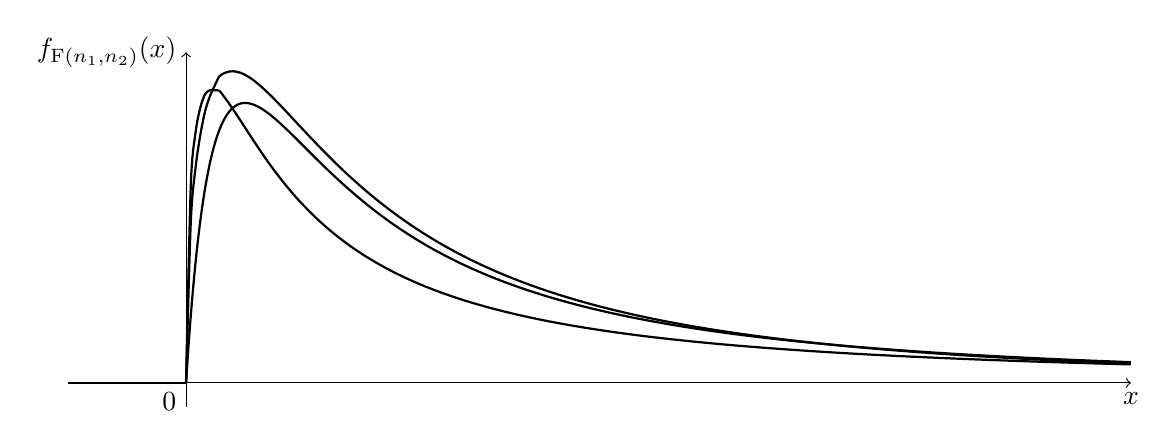
\begin{tikzpicture}[yscale = 6, xscale = 3, baseline={(current bounding box.center)}]
        \pgfmathsetmacro{\a}{3.30797337253}; % n1 = 3, n2 = 1
        \pgfmathsetmacro{\b}{64}; % n1 = 4, n2 = 2
        \pgfmathsetmacro{\c}{68.7549354157}; % n = 1
    
        \draw [->] (-0.5, 0) -- (4, 0);
        \draw [->] (0, -0.05) -- (0, 0.7);
        \draw [domain=0:4, smooth, variable = \x, thick, samples = 200] plot ({\x}, {\a*((\x)^(3/2 - 1))/(3*\x + 1)^((3+1)/2)});
        \draw [domain=0:4, smooth, variable = \x, thick, samples = 400] plot ({\x}, {\b*((\x)^(4/2 - 1))/(4*\x + 2)^((4+2)/2)});
        \draw [domain=0:4, smooth, variable = \x, thick, samples = 200] plot ({\x}, {\c*((\x)^(3/2 - 1))/(3*\x + 3)^((3+3)/2)});
        \node [below] at (4, 0) {$x$};
        \draw [thick] (-0.5, 0) -- (0, 0);
        \node [left] at (0, 0.7) {$f_{\mathrm{F}(n_1, n_2)}(x)$};
        \node [below left] at (0, 0) {$0$};
    \end{tikzpicture} 
\end{center}

\noindent\textbf{Числові характеристики:}
\begin{enumerate}
    \item $E\mathrm{F}(n_1, n_2) = \frac{n_2}{n_2 - 2}$, $n_2 > 2$.
    \item $D\mathrm{F}(n_1, n_2) = \frac{2 n_2^2 (n_1 + n_2 - 2)}{n_1 (n_2 - 2)^2 (n_2 -4)}$, $n_2>4$.
\end{enumerate}

\begin{remark}
    Якщо $\eta \sim \mathrm{F}(n_1, n_2)$, то $\frac{1}{\eta} \sim \mathrm{F}(n_2, n_1)$.
\end{remark}